\section{Zalety funkcji sklejanych}
\begin{frame}{Zalety}
	\begin{itemize}
	\item dokładniejsza, bezpieczniejsza interpolacja - patrz rysunek!
    \begin{figure}[h]
			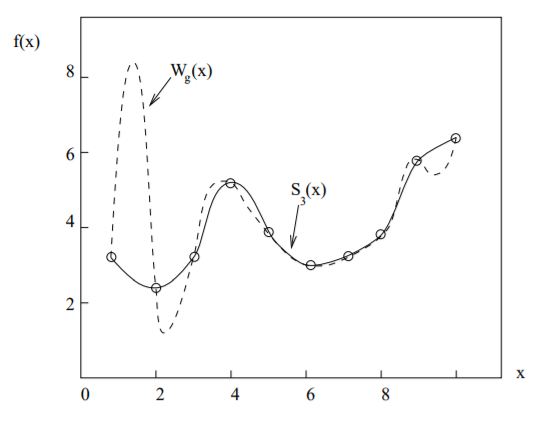
\includegraphics[width=.75\linewidth]{img/4/spline_img_5}
		\end{figure}
	\end{itemize}
\end{frame}
%%%%%%%%%%%%%%%%
\begin{frame}{Zalety c.d.}
	\begin{itemize}
		\item wartości $s_{3}(x)$ łatwe do wyznaczania
    	\item w praktyce - $s_{3}$ wystarczające
    	\item przydatne dla węzłów równoodległych
    	\item można używać dla określenia $\Rightarrow \frac{d^{(n)}}	
        	{dx^{n}}f(x)$
    		i $\int f(x)dx$ 
	\end{itemize}
	\begin{block}{Zadanie 1}
        	$s'(x), \ s''(x)$
    \end{block}
    \begin{block}{Zadanie 2}
        	$\int^{x_{n}}_{x_{1}}s(x)dx$
    \end{block}
\end{frame}
%%%%%%%%%%%%%%%%
\begin{frame}{Zastosowania}
	\begin{itemize}
		\item do wygładzania powierzchni:
        	\begin{itemize}
        		\item siatka porotokątna $(x_{i},y_{i})$, $i=1,2,...,m$; 
                	$j=0,1,...,n$
                \item funkcje sklejane na siatce, np.: 
                \[
                	\framebox{$s(x,y)=\sum_{i=0}^{m}\sum_{j=0}^{n}f(x_{i},
                    \ y_{i})\psi_{i}(x)\psi_{j}(y)$}
                \]
                %% dead link
        	\end{itemize}
	\end{itemize}
\end{frame}
%%%%changed encoding of file, utf-8 -> utf-8(without BOM)







